\chapter{Axiomas sobre medición de ángulos}

%---------- definición 3.1
\begin{tcolorbox}[colframe=white]
    \begin{def.}
	Un ángulo es la figura formada por dos semi-rectas que tiene el mismo origen. Su notación viene dado por $B\widehat{A}C$.
    \end{def.}
\end{tcolorbox}

%----------axioma 3.1
\begin{tcolorbox}[colframe=white]
    \begin{axioma}
	Cada ángulo tiene una medida mayor o igual a cero. La medida del ángulo es cero si y solo si está formada por dos semi-rectas coincidentes.\\\\
	A cada ángulo le corresponde un único número real mayor o igual a cero llamado medida del ángulo ($m A\widehat{O}B$).
    \end{axioma}
\end{tcolorbox}

%---------- definición 3.2
\begin{tcolorbox}[colframe=white]
    \begin{def.}
	Una semi-recta divide un semi-plano si ella está contenida en el semi-plano y su origen es un punto de la recta que lo determina.
    \end{def.}
\end{tcolorbox}

%----------axioma 3.2
\begin{tcolorbox}[colframe=white]
    \begin{axioma}
	Es posible colocar en correspondencia biunívoca los números reales entre $0$ y $180$ y las semi-rectas de mismo origen que dividen un semi-plano dado, de modo que la diferencia entre estos números sea la medida del ángulo formado por las semi-rectas correspondientes.\\\\
    \end{axioma}
\end{tcolorbox}

%---------- definición 3.3
\begin{tcolorbox}[colframe=white]
    \begin{def.}
	Sean $S_{OA}, S_{OB},S_{OC}$. Si el segmento $AB$ intersecta $S_{OC}$ diremos que $S_{OC}$ divide el ángulo $A\widehat{O}B$.
    \end{def.}
\end{tcolorbox}

%----------axioma 3.3
\begin{tcolorbox}[colframe=white]
    \begin{axioma}
	Si una semi-recta $S_{OC}$ divide un ángulo $A\widehat{O}B$ entonces $A\widehat{O}B = A\widehat{O}C + C\widehat{O}B$.
    \end{axioma}
\end{tcolorbox}

%---------- definición 3.4
\begin{tcolorbox}[colframe=white]
    \begin{def.}
	Dos ángulos se dicen suplementarios si la suma de sus medidas es $180^{\circ}$. El suplemento de un ángulo es el adyacente al ángulo dado obtenido por la prolongación de uno de sus lados.
    \end{def.}
\end{tcolorbox}

%---------- definición 3.5
\begin{tcolorbox}[colframe=white]
    \begin{def.}
	Si dos rectas distintas se intersectan, se forman cuatro ángulos.\\\\
	Decimos que $A\widehat{O}B$ y $C\widehat{O}D$ son opuestos por el vértice.
    \end{def.}
\end{tcolorbox}

    %----------proposición 3.1
    \begin{proposicion}
	Ángulos opuestos por el vértice tienen igual medida.\\\\
	    Demostración.-\; Sean $A\widehat{O}B + C\widehat{O}D $ opuestos por el vértice. Luego $$A\widehat{O}B + A\widehat{O}C = 180,$$ $$C\widehat{O}D + A\widehat{O}C = 180$$ Por lo tanto $A\widehat{O}B - C\widehat{O}D = 0$ y por lo tanto $A\widehat{O}B=C\widehat{O}D.$\\\\
    \end{proposicion}

    %----------teorema 3.1
    \begin{teo}
	Mostrar que dado el ángulo $A\widehat{O}B$, el suplemento de $A\widehat{O}B$ es un ángulo suplementario a $A\widehat{O}B$.\\\\
	    Demostración.-\; Sea $B\widehat{O}C$ suplemento de $A\widehat{O}B$. Supongamos que $S_{OA}=0$, $S_{OC}=180$ y $S_{OB} = b \in [0,180]$, luego $A\widehat{O}B = |0-b|=b$, $B\widehat{O}C = |180 - b| = 180-b$ y por lo tanto $A\widehat{O}B + B\widehat{O}C = 180$.\\\\
    \end{teo}


%---------- definición 3.6
\begin{tcolorbox}[colframe=white]
    \begin{def.}
	Un ángulo cuya medida es $90^{\circ}$ es llamado ángulo recto.\\\\
	Si dos rectas se intersectan y uno de los cuatro ángulos formados es recto, decimos que las rectas son perpendiculares.
    \end{def.}
\end{tcolorbox}

    %----------teorema 3.1
    \begin{teo}
	Por cualquier punto de una recta pasa una única perpendicular a esa recta.\\\\
	    Demostración.-\; (Existencia) Sea $m$ una recta y $A \in m$. Fijemos un semiplano que contiene a $m$. Por el axioma 3.2 existe $S_{AB}$ de coordenada $90^{\circ}$. Si tomamos $C$ en $m$, entonces o $B\widehat{A}C = |90-0|=90,$ o $B\widehat{A}C=|180-90|=90$ por tanto, la recta $AB$ es perpendicular a $m$.\\
	    (Unicidad) Sean $n,n^{'}$ rectas que pasan por $A$ y son perpendiculares a $m$. Trabajando en un semiplano, sea $\alpha$ la medida entre $n$ y $n^{'}$ y sean $\beta$ y $\lambda$. Como $n,n^{'}$ son perpendiculares a $m$ entonces $\beta, \lambda =90$, luego por el axioma 3.3 $\lambda + \alpha + \beta =180 \quad \Rightarrow \quad 180 + \alpha = 180 \quad \Rightarrow \quad \alpha = 0 $ de donde $n=n^{'}$.\\\\
    \end{teo}

\section{Ejercicios}

\begin{enumerate}[\Large\bfseries 1.]

	%--------------------1.
	\item Muestre que si un ángulo y su suplemento tienen la misma medida entonces el ángulo es recto.\\\\
	    Demostración.-\;  
	    \begin{center}
		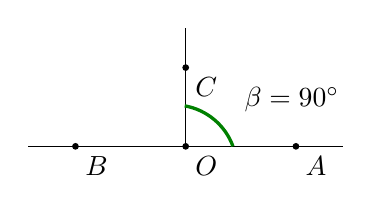
\begin{tikzpicture}
		    \draw(0,0)--(4,0);
		    \draw(2,0)--(2,1.5);
		    \draw [color=black](190:-3.4) node[rotate=0] {$\beta=90^{\circ}$};
		    \draw [green!50!black,very thick](0:2.6cm) arc (20:80:.8cm);
		    \filldraw[black](.6,0) circle(1pt) node[below right]{$B$};
		    \filldraw[black](2,0) circle(1pt) node[below right]{$O$};
		    \filldraw[black](2,1) circle(1pt) node[below right]{$C$};
		    \filldraw[black](3.4,0) circle(1pt) node[below right]{$A$};
		\end{tikzpicture}
	    \end{center}

	    Considere el ángulo $\alpha \; ó \; B \widehat{O} C$ y $\beta$, donde $\beta$ es el suplemento de $\alpha$. Por definición tenemos: $$ \alpha + \beta = 180^{\circ} \;\;\; (1)$$ como $\alpha = \beta$ entonces: $$\alpha + \alpha = 180^{\circ} \Rightarrow 2\alpha = 180^{\circ} \Rightarrow \alpha = 90^{\circ}$$ Luego por $(1)$ se concluye que $\beta = 90^{\circ}$.\\\\

	%--------------------2.
	\item Un ángulo es llamado agudo si mide menos de $90^{\circ}$, y es llamado obtuso si mide más de $90^{\circ}$. Muestre que el suplemento de un ángulo es siempre obtuso.\\\\
	    Demostración.-\; Sea $\alpha$ un ángulo agudo y $\beta$  el suplemento de $\alpha$. Sabemos que $\alpha + \beta = 180^{\circ}$ y $\alpha < 90^{\circ}$ y $\beta = 180^{\circ} - \alpha$ entonces $\beta > 90^{\circ}$ como queríamos demostrar demostrar.\\\\

	%--------------------3.
	\item Dos ángulos se dicen complementarios si su suma es un ángulo recto. Dos ángulos son complementarios y el suplemento de un de ellos mide tanto como el suplemento del segundo más $30^{\circ}$. ¿Cuánto miden los dos ángulos?\\\\
	    Demostración.-\; Sea $\alpha + \beta = 90^{\circ}\;\; (1)$ con $\alpha_1 y \beta_1$ suplementos de $\alpha$ y $\beta$ entonces: $$\alpha + \alpha_1\;\; (2)$$ 
	    $$\beta + \beta_1\;\; (3)$$ luego haciendo $\alpha_1 = \beta_1 + 30^{\circ}\;\; (4)$ es decir, un ángulo igual a otro sumando $30$ grados. Y reemplazando $\beta_1$ de $(3)$ en $(4)$ entonces: 
	    $$\alpha_1 = (180^{\circ} - \beta) + 30^{\circ} = 210^{\circ} - \beta \;\; (5)$$ De donde reemplazando $(5)$ en $(2)$ 
	    $$\alpha + 210^{\circ} - \beta = 180^{\circ}$$ 
	    $$\alpha - \beta = -30^{\circ}\;\; (6)$$ de las ecuaciones $(1)$ y $(6)$ configuramos el sistema:\\
	    Cuya solución es $\alpha = 30^{\circ} y \beta = 60^{\circ}$, por lo que un ángulo posible tiene $30$ y otros $60$ grados.\\\\

	%--------------------4.
	\item Una poligonal es una figura formada por una sucesión de puntos $A_1,A_2,...,A_n$ y por los segmentos $A_1A_2,A_2A_3,...,A_{n-1}A_n$. Los puntos son los vértices de la poligonal y los segmentos son sus lados. Diseñe una poligonal $ABCD$ sabiendo que; $AB=BC=CD=2cm$, $ABC=120$ y $BCD=100$.\\\\
	Respuesta.-\; 

	    \begin{center}
		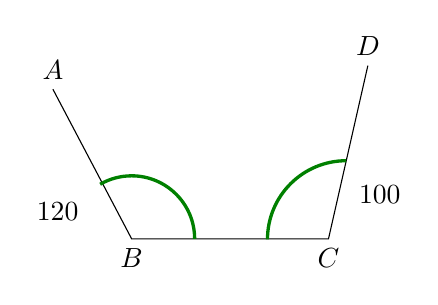
\begin{tikzpicture}
		    \draw(-1,1.9)node[above]{$A$}--(0,0)node[below]{$B$}--(2.5,0)node[below]{$C$}--(3,2.2)node[above]{$D$};
		    \draw [color=black](160:1) node[rotate=0] {$120$};
		    \draw [green!50!black,very thick](0:.8cm) arc (0:120:.8cm);
		    \draw [color=black](10:3.2) node[rotate=0] {$100$};
		    \draw [green!50!black,very thick](20:2.9cm) arc (90:180:1cm);
		\end{tikzpicture}
	    \end{center}

	%--------------------5.
	\item Un polígono es una poligonal que satisface las siguientes tres condiciones.
	    \begin{enumerate}[\bfseries a)]

		%----------a)
		\item $A_n=A_1$

		%----------b)
		\item los lados de la poligonal se intersectan solamente en sus extremos y, 

		%----------c)
		\item dos lados con un mismo extremo no pertenecen a una misma recta. 
	    \end{enumerate}
	de las 4 figuras siguientes, apenas dos son polígonos. Determine cuales son.

	    \begin{multicols}{2}
		\begin{center}
		    \begin{tikzpicture}
			\draw(.2,0)node[below]{\tiny$A$}--(1.8,.8)node[below]{\tiny$B$}--(1,1.9)node[above]{\tiny$C$}--(-.6,2.3)node[above]{\tiny$D$}--(-1.6,1.1)node[left]{\tiny$E$}--(.2,0);
		    \end{tikzpicture}
		    
		    \begin{tikzpicture}
			\draw(0,0)node[left]{\tiny$A$}--(1.5,0)node[below]{\tiny$E$}--(2.5,0)node[right]{\tiny$D$}--(2.8,1.8)node[above]{\tiny$C$}--(0,0);
		    \end{tikzpicture}

		    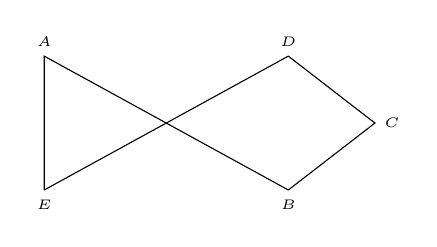
\begin{tikzpicture}
			\draw(.4,0)node[below]{\tiny $E$}--(.4,1.7)node[above]{\tiny $A$}--(3.5,0)node[below]{\tiny $B$}--(4.6,0.85)node[right]{\tiny $C$}--(3.5,1.7)node[above]{\tiny $D$}--(.4,0);
		    \end{tikzpicture}

		    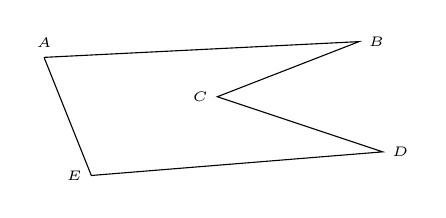
\begin{tikzpicture}
			\draw(0,0)node[above]{\tiny $A$}--(4,0.2)node[right]{\tiny $B$}--(2.2,-.5)node[left]{\tiny $C$}--(4.3,-1.2)node[right]{\tiny $D$}--(.6,-1.5)node[left]{\tiny $E$}--(0,0);
		    \end{tikzpicture}
		\end{center}
	    \end{multicols}
	    Un polígono de vértices $A_1,A_2,...,A_{n+1}=A_1$, se denotará por $A_1,A_2...A_n$; él tiene $n$ lados y $n$ ángulos.\\\\

	    Respuesta.-\; La primera figura a la izquierda y en la línea superior es un polígono. El segundo desde la izquierda, también desde la línea superior no lo es, porque si lo fuera, contradiría la segunda condición. El primero a la izquierda de la línea inferior tampoco es un polígono, ya que iría en contra de la tercera condición.Y por último el segundo en la fila inferior es un polígono.\\\\
 
	%--------------------6.
	\item Diseñe un polígono de 4 lados $ABCD$ tal que $AB=BC=CD=DA=2cm$, con $ABC=ADC=100$ y con $BCD=BAD=80$.\\\\
	Respuesta.-\; 

	\begin{center}
	    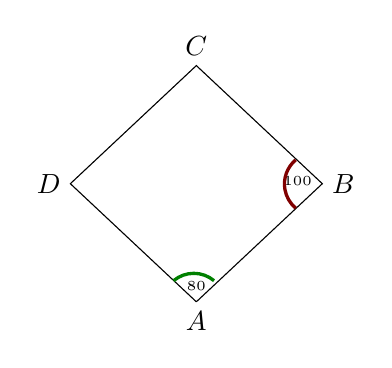
\begin{tikzpicture}
		\draw(0,0)node[below]{$A$}--(1.6,1.5)node[right]{$B$}--(0,3)node[above]{$C$}--(-1.6,1.5)node[left]{$D$}--(0,0);
		\draw [color=black](90:.2) node[rotate=0] {\tiny$80$};
		\draw [green!50!black,very thick](50:.35cm) arc (50:130:.4cm);
		\draw [color=black](50:2cm) node[rotate=0] {\tiny$100$};
		\draw [red!50!black,very thick](55:2.2cm) arc (130:230:.4cm);
	    \end{tikzpicture}
	\end{center}

	%--------------------7.
	\item El segmento que une dos vértices no consecutivos de un polígono es llamado una diagonal del polígono. Haga un diseño de un polígono de seis lados, luego diseñe todas las diagonales. ¿Cuántas diagonales tendrá un polígono de $20$ lados? ¿Y, de $n$ lados?\\\\
	Respuesta.-\; Tenemos un polígono de 6 lados:
	\begin{center}
	    \begin{tikzpicture}
		\draw(0,0)node[below]{$A$}--(1.8,1)node[right]{$B$}--(1.8,3)node[right]{$C$}--(0,4)node[above]{$D$}--(-1.8,3)node[left]{$E$}--(-1.8,1)node[left]{$F$}--(0,0);
	    \end{tikzpicture}
	\end{center}
	    Desde el vértice $A$, por ejemplo, debería comenzar en diagonal para todos los demás vértices excepto para él mismo y para los otros dos adyacentes. Como tenemos 6 vértices, desde el punto $A$ un total de: $6-3$ diagonal.

	\begin{center}
	    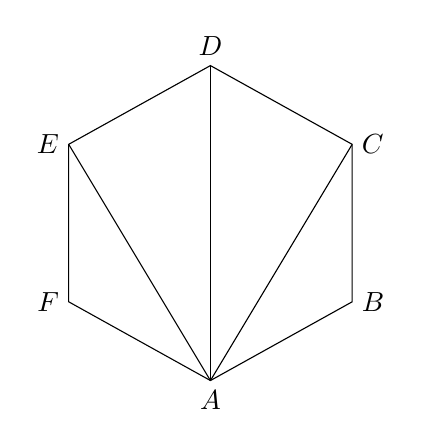
\begin{tikzpicture}
		\draw(0,0)node[below]{$A$}--(1.8,1)node[right]{$B$}--(1.8,3)node[right]{$C$}--(0,4)node[above]{$D$}--(-1.8,3)node[left]{$E$}--(-1.8,1)node[left]{$F$}--(0,0);
		\draw(0,0)--(1.8,3);
		\draw(0,0)--(-1.8,3);
		\draw(0,0)--(0,4);
	    \end{tikzpicture}
	\end{center}
	    Lo mismo ocurre con los otros vértices. Entonces, si tenemos seis vértices, tendremos en total $(6 - 3) · 6 =$ diagonales.

	\begin{center}
	    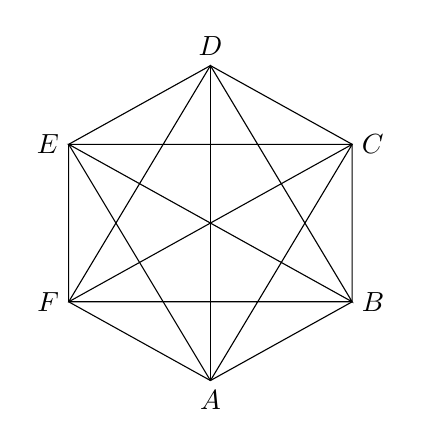
\begin{tikzpicture}
		\draw(0,0)node[below]{$A$}--(1.8,1)node[right]{$B$}--(1.8,3)node[right]{$C$}--(0,4)node[above]{$D$}--(-1.8,3)node[left]{$E$}--(-1.8,1)node[left]{$F$}--(0,0);
		\draw(0,0)--(1.8,3)--(-1.8,3)--(1.8,1)--(0,4)--(-1.8,1)--(1.8,1);
		\draw(0,0)--(-1.8,3);
		\draw(0,0)--(0,4);
		\draw(-1.8,1)--(1.8,3);
	    \end{tikzpicture}
	\end{center}
	    Sin embargo la diagonal $AB$ es también la diagonal $BA$ y lo mismo ocurre con las otras diagonales que acaban contando dos veces. Considerando este hecho en el número total de diagonales, será: $$\dfrac{(6 - 3) 6}{2} = 9$$ Para un polígono de $n$ lados, entonces tendríamos: $$\dfrac{(n - 3)n}{2}$$ Esta fórmula se puede usar para determinar el número de vértices de cualquier polígono, como el de $20$ lados qué tendría $$\dfrac{(20 - 3) 20}{2} = 170 \; lados.$$\\\\

	%--------------------8.
	\item Un polígono es convexo si siempre está contenido en uno de los semiplanos determinados por las rectas que contienen a sus lados. En la figura siguiente el polígono a) es convexo y el b) no es convexo. Justifique

	    \begin{multicols}{2}
		\begin{center}
		    \begin{tikzpicture}
			\draw(0,0)--(2.8,0)--(2.9,1.8)--(0,2.5)--(-1,1)--(0,0);
			\draw(1,0)node[below]{$a)$};
		    \end{tikzpicture}
		    
		    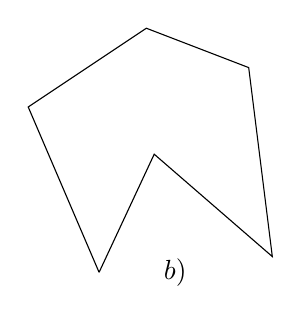
\begin{tikzpicture}
			\draw(0,0)--(.7,1.5)--(2.2,0.2)--(1.9,2.6)--(.6,3.1)--(-.9,2.1)--(0,0);
			\draw(.7,0)node[right]{$b)$};
		    \end{tikzpicture}
		\end{center}
	    \end{multicols}
	    Los polígonos convexos reciben nombres especiales. Se dan las designaciones de estos polígonos de acuerdo a su número de lados, hasta 10 lados.
	    \begin{center}
		\begin{tabular}{cc}
		    n de lados  &  nombre del polígono convexo\\
		    \hline
		     3 & triángulo \\
		     4 & cuadrilátero\\
		     5 & pentágono\\
		     6 & hexágono\\
		     7 & heptágano\\
		     8 & octágono\\
		     9 & nonagono\\
		     10& decágono\\
		\end{tabular}
	    \end{center}
	    
	%--------------------9.
	\item Describa un método, en que se haga uso de un compás y una regla no numerada, de construcción de un cuadrilátero con los cuatro lados de misma longitud. Extienda su método para el caso de 5 lados.\\\\
	Respuesta.-\; Dibuja un círculo con radio $r$ y centro en $O$, y en cualquier punto del círculo marca un punto.

	\begin{center}
	    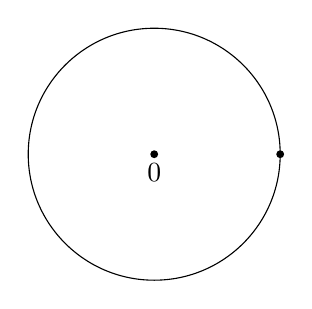
\begin{tikzpicture}[scale=.8]
		\draw(0,0) circle (2cm);
		\filldraw[black](0,0) circle(1.5pt) node[below]{$0$};
		\filldraw[black](2,0) circle(1.5pt);
	    \end{tikzpicture}
	\end{center}

	Ahora convertimos el punto escogido en la circunferencia como punto medio de un segundo circulo.

	\begin{center}
	    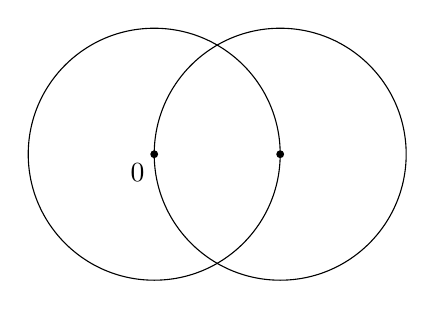
\begin{tikzpicture}[scale=.8]
		\draw(0,0) circle (2cm);
		\draw(2,0) circle (2cm);
		\filldraw[black](0,0) circle(1.5pt) node[below left]{$0$};
		\filldraw[black](2,0) circle(1.5pt);
	    \end{tikzpicture}
	\end{center}

	Marque de nuevo otro punto en la intersección de los círculos como en en la figura.

	\begin{center}
	    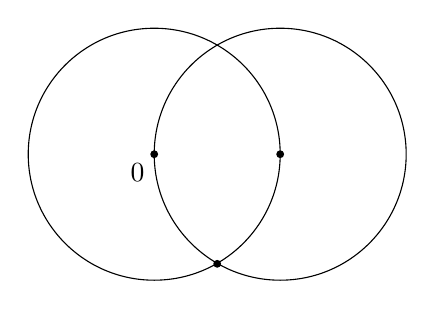
\begin{tikzpicture}[scale=.8]
		\draw(0,0) circle (2cm);
		\draw(2,0) circle (2cm);
		\filldraw[black](0,0) circle(1.5pt) node[below left]{$0$};
		\filldraw[black](2,0) circle(1.5pt);
		\filldraw[black](1,-1.74) circle(1.5pt);
	    \end{tikzpicture}
	\end{center}

	Y con el compás, aún con la misma medida, dibuja un nuevo círculo centrado en el último punto esbozado.

	\begin{center}
	    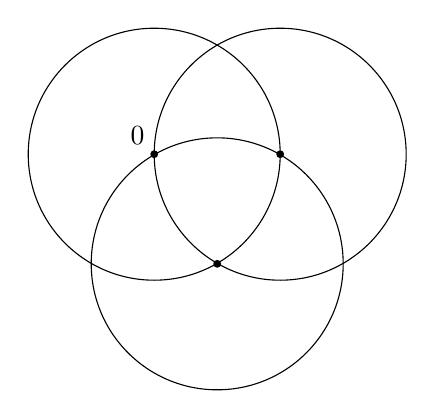
\begin{tikzpicture}[scale=.8]
		\draw(0,0) circle (2cm);
		\draw(2,0) circle (2cm);
		\draw(1,-1.74) circle (2cm);
		\filldraw[black](0,0) circle(1.5pt) node[above left]{$0$};
		\filldraw[black](2,0) circle(1.5pt);
		\filldraw[black](1,-1.74) circle(1.5pt);
	    \end{tikzpicture}
	\end{center}

	Finalmente tracemos segmentos entre todos los puntos de intersección.

	\begin{center}
	    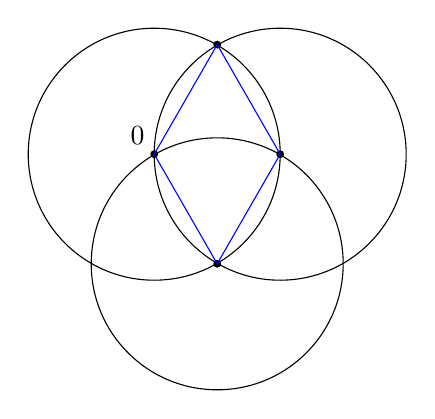
\begin{tikzpicture}[scale=.8]
		\draw(0,0) circle (2cm);
		\draw(2,0) circle (2cm);
		\draw(1,-1.74) circle (2cm);
		\filldraw[black](0,0) circle(1.5pt) node[above left]{$0$};
		\filldraw[black](2,0) circle(1.5pt);
		\filldraw[black](1,-1.74) circle(1.5pt);
		\filldraw[black](1,1.74) circle(1.5pt);
		\draw[blue](1,1.74)--(0,0)--(1,-1.74)--(2,0)--(1,1.74);
	    \end{tikzpicture}
	\end{center}

	Haciendo cuatro segmentos de longitud $r$.

	\begin{center}
	    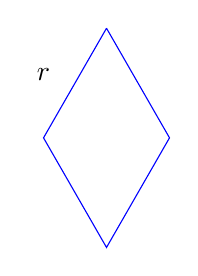
\begin{tikzpicture}[scale=.8]
		\draw[blue](1,1.74)--(0,0)--(1,-1.74)--(2,0)--(1,1.74);
		\draw(0,1)node[]{$r$};
	    \end{tikzpicture}
	\end{center}

	Luego generalizando.\\
	Dibuja un círculo con radio r y centro en o, y en cualquier punto del círculo marca un punto.

	\begin{center}
	    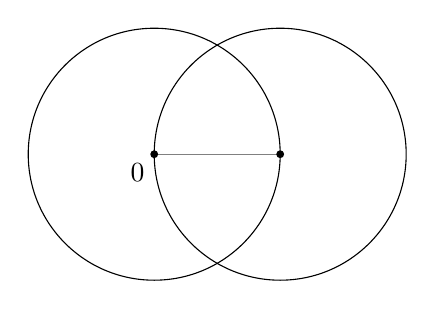
\begin{tikzpicture}[scale=.8]
		\draw(0,0) circle (2cm);
		\draw(2,0) circle (2cm);
		\draw[gray](0,0)--(2,0);
		\filldraw[black](0,0) circle(1.5pt) node[below left]{$0$};
		\filldraw[black](2,0) circle(1.5pt);
	    \end{tikzpicture}
	\end{center}

	Ahora marque un nuevo punto como en el segundo círculo para que no esté en la misma línea que los otros dos. Más o menos como en la figura a continuación:

	\begin{center}
	    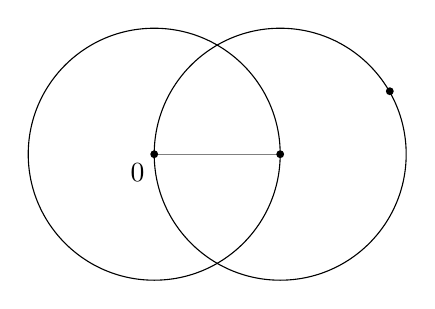
\begin{tikzpicture}[scale=.8]
		\draw(0,0) circle (2cm);
		\draw(2,0) circle (2cm);
		\draw[gray](0,0)--(2,0);
		\filldraw[black](0,0) circle(1.5pt) node[below left]{$0$};
		\filldraw[black](2,0) circle(1.5pt);
		\filldraw[black](3.74,1) circle(1.5pt);
	    \end{tikzpicture}
	\end{center}
	
	Dibujamos un nuevo círculo con el mismo radio $r$, centrado en el punto. Así formando un nuevo segmento.

	\begin{center}
	    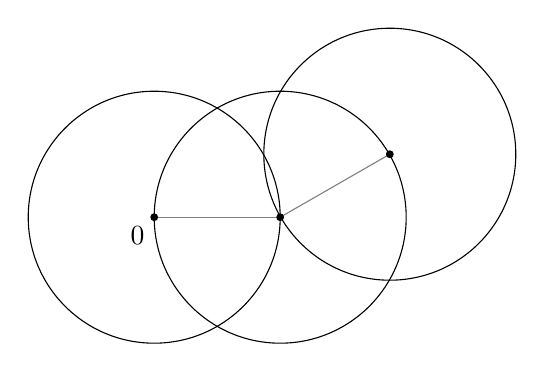
\begin{tikzpicture}[scale=.8]
		\draw(0,0) circle (2cm);
		\draw(2,0) circle (2cm);
		\draw(3.74,1) circle (2cm);
		\draw[gray](0,0)--(2,0);
		\draw[gray](2,0)--(3.74,1);
		\filldraw[black](0,0) circle(1.5pt) node[below left]{$0$};
		\filldraw[black](2,0) circle(1.5pt);
		\filldraw[black](3.74,1) circle(1.5pt);
	    \end{tikzpicture}
	\end{center}

	Repitiendo el proceso, se dibuja un nuevo círculo y se dibuja un nuevo punto.

	\begin{center}
	    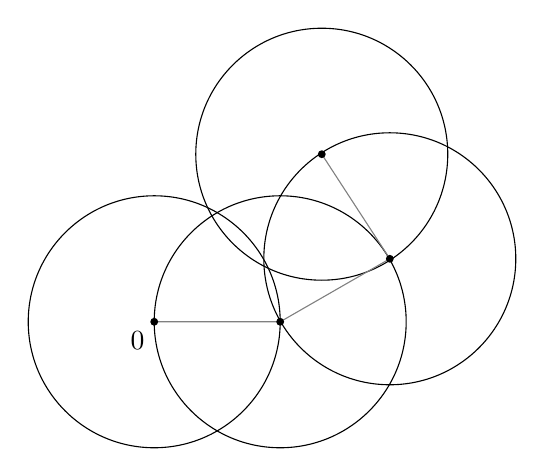
\begin{tikzpicture}[scale=.8]
		\draw(0,0) circle (2cm);
		\draw(2,0) circle (2cm);
		\draw(3.74,1) circle (2cm);
		\draw(2.66,2.66) circle (2cm);
		\draw[gray](0,0)--(2,0)--(3.74,1)--(2.66,2.66);
		\filldraw[black](0,0) circle(1.5pt) node[below left]{$0$};
		\filldraw[black](2,0) circle(1.5pt);
		\filldraw[black](3.74,1) circle(1.5pt);
		\filldraw[black](2.66,2.66) circle(1.5pt);
	    \end{tikzpicture}
	\end{center}

	En la intersección entre el último (azul) y el primer círculo dibujado (rojo), marcamos un punto (que llamaremos $P$).

	\begin{center}
	    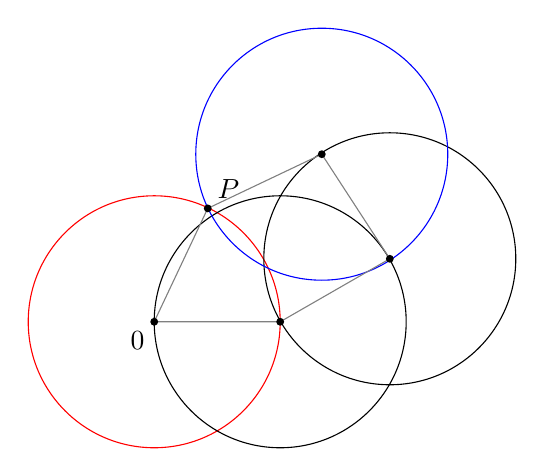
\begin{tikzpicture}[scale=.8]
		\draw[red](0,0) circle (2cm);
		\draw(2,0) circle (2cm);
		\draw(3.74,1) circle (2cm);
		\draw[blue](2.66,2.66) circle (2cm);
		\draw[gray](0,0)--(2,0)--(3.74,1)--(2.66,2.66)--(.85,1.8)--(0,0);
		\filldraw[black](0,0) circle(1.5pt) node[below left]{$0$};
		\filldraw[black](2,0) circle(1.5pt);
		\filldraw[black](3.74,1) circle(1.5pt);
		\filldraw[black](2.66,2.66) circle(1.5pt);
		\filldraw[black](.85,1.8) circle(1.5pt) node[above right]{$P$};
	    \end{tikzpicture}
	\end{center}

	Esto formará un polígono de 5 lados cada uno con una longitud igual a $r$.

	\begin{center}
	    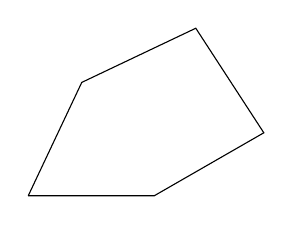
\begin{tikzpicture}[scale=.8]
		\draw(0,0)--(2,0)--(3.74,1)--(2.66,2.66)--(.85,1.8)--(0,0);
	    \end{tikzpicture}
	\end{center}
	\vspace{1cm}

	%--------------------10.
    \item Dado un ángulo $A \widehat{O} B$ muestre que existe una única semirecta $S_{OC}$ tal que $A \widehat{O} C=C \widehat{O} B$. La semirecta $S_{OC}$ es llamada bisectriz del ángulo $A \widehat{O}B$\\\\
	Demostración.-\; Considere un ángulo $A \widehat{O} B$ con bisectriz $S_{OC}$.

	\begin{center}
	    \begin{tikzpicture}
		\draw[->](0,0)node[below]{$O$}--(2,0)node[right]{$B$};
		\filldraw[black](1.5,0) circle(1.5pt);
		\draw[->](0,0)--(1.5,1.8)node[right]{$C$};
		\filldraw[black](1.25,1.5) circle(1.5pt);
		\draw[->](0,0)--(-1,1.5)node[left]{$A$};
		\filldraw[black](-.8,1.2) circle(1.5pt);
	    \end{tikzpicture}
	\end{center}

	Supongamos que hay una segunda bisectriz $S_{OC} \neq  S_{OC}$ que también es bisectriz de $AOB$. En este caso, existen dos posibilidades:

	\begin{enumerate}[\bfseries i.]

	    \item $S_{OC^{'}}$ está a la derecha de $S_{OC}$, como siguiente.

	    \begin{center}
		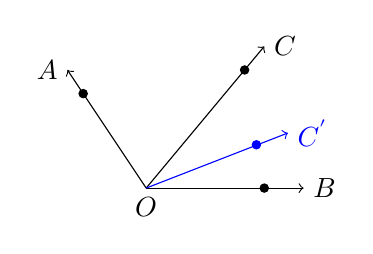
\begin{tikzpicture}
		    \draw[->](0,0)node[below]{$O$}--(2,0)node[right]{$B$};
		    \filldraw[black](1.5,0) circle(1.5pt);
		    \draw[->](0,0)--(1.5,1.8)node[right]{$C$};
		    \filldraw[black](1.25,1.5) circle(1.5pt);
		    \draw[->](0,0)--(-1,1.5)node[left]{$A$};
		    \filldraw[black](-.8,1.2) circle(1.5pt);
		    \draw[->, blue](0,0)--(1.8,0.7)node[right]{$C^{'}$};
		    \filldraw[blue](1.4,.55) circle(1.5pt);
		\end{tikzpicture}
	    \end{center}

	    \item o $S_{OC^{'}}$ está a la izquierda de $S_{OC}$. 

	    \begin{center}
		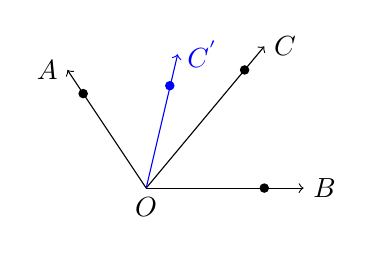
\begin{tikzpicture}
		    \draw[->](0,0)node[below]{$O$}--(2,0)node[right]{$B$};
		    \filldraw[black](1.5,0) circle(1.5pt);
		    \draw[->](0,0)--(1.5,1.8)node[right]{$C$};
		    \filldraw[black](1.25,1.5) circle(1.5pt);
		    \draw[->](0,0)--(-1,1.5)node[left]{$A$};
		    \filldraw[black](-.8,1.2) circle(1.5pt);
		    \draw[->, blue](0,0)--(.4,1.7)node[right]{$C^{'}$};
		    \filldraw[blue](.3,1.3) circle(1.5pt);
		\end{tikzpicture}
	    \end{center}
	\end{enumerate}

	Consideremos el caso $I$.\\
	Como $S_{OC^{'}}$  y $S_{OC}$ son bisectrices de $A\widehat{O}B$, entonces según el axioma $III_6$,
	 \begin{center}
	     \begin{tabular}{rclclc}
		 $A\widehat{O}B$ & $=$ & $A\widehat{O}C + C\widehat{O}B$ & $=$ & $2C \widehat{O}B$ & $(1)$ \\
		 $A\widehat{O}B$ & $=$ & $A\widehat{O}C^{'} + C^{'}\widehat{O}B$ & $=$ & $2C^{'}\widehat{O}B$ & $(2)$ \\
	     \end{tabular}
	\end{center}

	La figura $2$ muestra que $COB = COC^{'} + C^{'}OB \;\; (3)$, luego remplazamos $(3)$ en $(1)$
	$$A\widehat{O}B = 2(C\widehat{O}C + C^{'}\widehat{O}B) \,\,\, (4)$$
	Así igualando $(2)$ y $(4)$
	\begin{center}
	    \begin{tabular}{c r c l}
		&$A\widehat{O}B$&$=$&$A\widehat{O}B$\\
		&$2C^{'}\widehat{O}B$&$=$&$2C\widehat{O}C + 2 C^{'}\widehat{O}B$\\
		$\Rightarrow$&$C\widehat{O}C^{'}$&$=$&$0$\\
	    \end{tabular}
	\end{center}

	Sin embargo, si $C\widehat{O}C^{'}=0$ entonces por el axioma $III_4$ $S_OC = S_{OC^{'}}$ que contradice la hipótesis inicial de que $S_{OC} = S_{OC^{'}}$. Por lo tanto, el ángulo $A\widehat{O}B$ no puede tener más de una bisectriz. De manera similar para el caso de $S_{OC^{'}}$  a la izquierda de $S_{OC}$\\\\

	%--------------------11.
	\item Muestre que la bisectrices de un ángulo y de su suplemento son perpendiculares.\\\\
	Demostración.-\; Sea
	\begin{center}
	    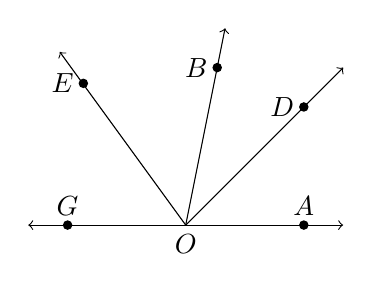
\begin{tikzpicture}
		\draw[<->](0,0)--(4,0);
		\draw[->](2,0)node[below]{$O$}--(4,2);
		\draw[->](2,0)--(2.5,2.5);
		\draw[->](2,0)--(0.4,2.2);
		\filldraw[black](.5,0) circle(1.5pt) node[above]{$G$};
		\filldraw[black](3.5,0) circle(1.5pt) node[above]{$A$};
		\filldraw[black](3.5,1.5) circle(1.5pt) node[left]{$D$};
		\filldraw[black](2.4,2) circle(1.5pt) node[left]{$B$};
		\filldraw[black](.7,1.8) circle(1.5pt) node[left]{$E$};

	    \end{tikzpicture}
	\end{center}
	Sea $A\widehat{O}B$ un ángulo y $B\widehat{O}C$ su suplemento, entonces: $$A\widehat{O}B + B\widehat{O}C = 180^{\circ}\,\,\, (1)$$ Queremos mostrar que $B\widehat{O}D + B\widehat{O}E = 90^{\circ}$ para esto, tenga en cuenta que $B\widehat{O}D = \dfrac{A\widehat{O}B}{2},$ por lo tanto, $S_{OD}$ es la bisectriz de $A\widehat{O}B$ y $B\widehat{O}E = \dfrac{B\widehat{O}C}{2}$ luego, $B\widehat{O}E + B\widehat{O}D = \dfrac{A\widehat{O}B}{2} + \dfrac{B\widehat{O}C}{2}\,\,\, (2)$\\ 
	Igualando $(1)$ y $(2)$, 
	\begin{center}
	    \begin{tabular}{rcccl}
		$2(B\widehat{O}E + B\widehat{O}D)$ & $=$ & $A\widehat{O}B + B\widehat{O}C$ & $=$ & $180^{\circ}$\\
		$B\widehat{O}E + B\widehat{O}D$ & $=$ & $\dfrac{180^{\circ}}{2}$ & $=$ & $90^{\circ}$\\ 
	    \end{tabular}
	\end{center}

	Lo que implica que $S_{OE} \perp S_{OD}$ como queríamos demostrar.\\\\

	%--------------------12.
	\item Dado un ángulo $A\widehat{O}B$ y un número real positivo $a,$ $0<a<1$, muestre que existe una única semirecta $S_{OC}$ tal que $C \widehat{O}B=a,$ $A \widehat{O} B$\\\\
	Demostración.-\; Esta afirmación no es cierta, sin embargo se puede probar si también se pone la condición de que $C$ debe estar entre $A$ y $B$.\\\\


\end{enumerate}
